\documentclass[twoside]{book}

% Packages required by doxygen
\usepackage{fixltx2e}
\usepackage{calc}
\usepackage{doxygen}
\usepackage[export]{adjustbox} % also loads graphicx
\usepackage{graphicx}
\usepackage[utf8]{inputenc}
\usepackage{makeidx}
\usepackage{multicol}
\usepackage{multirow}
\PassOptionsToPackage{warn}{textcomp}
\usepackage{textcomp}
\usepackage[nointegrals]{wasysym}
\usepackage[table]{xcolor}

% Font selection
\usepackage[T1]{fontenc}
\usepackage[scaled=.90]{helvet}
\usepackage{courier}
\usepackage{amssymb}
\usepackage{sectsty}
\renewcommand{\familydefault}{\sfdefault}
\allsectionsfont{%
  \fontseries{bc}\selectfont%
  \color{darkgray}%
}
\renewcommand{\DoxyLabelFont}{%
  \fontseries{bc}\selectfont%
  \color{darkgray}%
}
\newcommand{\+}{\discretionary{\mbox{\scriptsize$\hookleftarrow$}}{}{}}

% Page & text layout
\usepackage{geometry}
\geometry{%
  a4paper,%
  top=2.5cm,%
  bottom=2.5cm,%
  left=2.5cm,%
  right=2.5cm%
}
\tolerance=750
\hfuzz=15pt
\hbadness=750
\setlength{\emergencystretch}{15pt}
\setlength{\parindent}{0cm}
\setlength{\parskip}{3ex plus 2ex minus 2ex}
\makeatletter
\renewcommand{\paragraph}{%
  \@startsection{paragraph}{4}{0ex}{-1.0ex}{1.0ex}{%
    \normalfont\normalsize\bfseries\SS@parafont%
  }%
}
\renewcommand{\subparagraph}{%
  \@startsection{subparagraph}{5}{0ex}{-1.0ex}{1.0ex}{%
    \normalfont\normalsize\bfseries\SS@subparafont%
  }%
}
\makeatother

% Headers & footers
\usepackage{fancyhdr}
\pagestyle{fancyplain}
\fancyhead[LE]{\fancyplain{}{\bfseries\thepage}}
\fancyhead[CE]{\fancyplain{}{}}
\fancyhead[RE]{\fancyplain{}{\bfseries\leftmark}}
\fancyhead[LO]{\fancyplain{}{\bfseries\rightmark}}
\fancyhead[CO]{\fancyplain{}{}}
\fancyhead[RO]{\fancyplain{}{\bfseries\thepage}}
\fancyfoot[LE]{\fancyplain{}{}}
\fancyfoot[CE]{\fancyplain{}{}}
\fancyfoot[RE]{\fancyplain{}{\bfseries\scriptsize Generated by Doxygen }}
\fancyfoot[LO]{\fancyplain{}{\bfseries\scriptsize Generated by Doxygen }}
\fancyfoot[CO]{\fancyplain{}{}}
\fancyfoot[RO]{\fancyplain{}{}}
\renewcommand{\footrulewidth}{0.4pt}
\renewcommand{\chaptermark}[1]{%
  \markboth{#1}{}%
}
\renewcommand{\sectionmark}[1]{%
  \markright{\thesection\ #1}%
}

% Indices & bibliography
\usepackage{natbib}
\usepackage[titles]{tocloft}
\setcounter{tocdepth}{3}
\setcounter{secnumdepth}{5}
\makeindex

% Hyperlinks (required, but should be loaded last)
\usepackage{ifpdf}
\ifpdf
  \usepackage[pdftex,pagebackref=true]{hyperref}
\else
  \usepackage[ps2pdf,pagebackref=true]{hyperref}
\fi
\hypersetup{%
  colorlinks=true,%
  linkcolor=blue,%
  citecolor=blue,%
  unicode%
}

% Custom commands
\newcommand{\clearemptydoublepage}{%
  \newpage{\pagestyle{empty}\cleardoublepage}%
}

\usepackage{caption}
\captionsetup{labelsep=space,justification=centering,font={bf},singlelinecheck=off,skip=4pt,position=top}

%===== C O N T E N T S =====

\begin{document}

% Titlepage & ToC
\hypersetup{pageanchor=false,
             bookmarksnumbered=true,
             pdfencoding=unicode
            }
\pagenumbering{roman}
\begin{titlepage}
\vspace*{7cm}
\begin{center}%
{\Large Robust View-\/\+Graph S\+L\+AM }\\
\vspace*{1cm}
{\large Generated by Doxygen 1.8.11}\\
\end{center}
\end{titlepage}
\clearemptydoublepage
\tableofcontents
\clearemptydoublepage
\pagenumbering{arabic}
\hypersetup{pageanchor=true}

%--- Begin generated contents ---
\chapter{Hierarchical Index}
\section{Class Hierarchy}
This inheritance list is sorted roughly, but not completely, alphabetically\+:\begin{DoxyCompactList}
\item \contentsline{section}{epnp}{\pageref{classepnp}}{}
\item exception\begin{DoxyCompactList}
\item \contentsline{section}{Exception}{\pageref{classException}}{}
\begin{DoxyCompactList}
\item \contentsline{section}{Invalid\+Operation\+Exception}{\pageref{classInvalidOperationException}}{}
\item \contentsline{section}{Null\+Pointer\+Exception}{\pageref{classNullPointerException}}{}
\end{DoxyCompactList}
\end{DoxyCompactList}
\item \contentsline{section}{Feature\+Selector}{\pageref{classFeatureSelector}}{}
\item \contentsline{section}{Graph\+Optimiser}{\pageref{classGraphOptimiser}}{}
\item \contentsline{section}{Image}{\pageref{classImage}}{}
\item \contentsline{section}{Pair}{\pageref{structPair}}{}
\item \contentsline{section}{Tracker\+:\+:point\+\_\+2d}{\pageref{structTracker_1_1point__2d}}{}
\item \contentsline{section}{Poly\+Matrix}{\pageref{classPolyMatrix}}{}
\item \contentsline{section}{Polynomial}{\pageref{classPolynomial}}{}
\item \contentsline{section}{Pwg\+Optimiser\+:\+:pulled\+\_\+constraint}{\pageref{structPwgOptimiser_1_1pulled__constraint}}{}
\item \contentsline{section}{Pwg\+Optimiser}{\pageref{classPwgOptimiser}}{}
\item \contentsline{section}{Recover\+Moments}{\pageref{classRecoverMoments}}{}
\item \contentsline{section}{Image\+:\+:Rgb}{\pageref{structImage_1_1Rgb}}{}
\item \contentsline{section}{Tracker}{\pageref{classTracker}}{}
\end{DoxyCompactList}

\chapter{Class Index}
\section{Class List}
Here are the classes, structs, unions and interfaces with brief descriptions\+:\begin{DoxyCompactList}
\item\contentsline{section}{\hyperlink{classepnp}{epnp} }{\pageref{classepnp}}{}
\item\contentsline{section}{\hyperlink{classException}{Exception} \\*\hyperlink{classException}{Exception} base class }{\pageref{classException}}{}
\item\contentsline{section}{\hyperlink{classFeatureSelector}{Feature\+Selector} }{\pageref{classFeatureSelector}}{}
\item\contentsline{section}{\hyperlink{classGraphOptimiser}{Graph\+Optimiser} }{\pageref{classGraphOptimiser}}{}
\item\contentsline{section}{\hyperlink{classImage}{Image} }{\pageref{classImage}}{}
\item\contentsline{section}{\hyperlink{classInvalidOperationException}{Invalid\+Operation\+Exception} \\*Invalid operation exception }{\pageref{classInvalidOperationException}}{}
\item\contentsline{section}{\hyperlink{classNullPointerException}{Null\+Pointer\+Exception} \\*Null pointer exception }{\pageref{classNullPointerException}}{}
\item\contentsline{section}{\hyperlink{structPair}{Pair} }{\pageref{structPair}}{}
\item\contentsline{section}{\hyperlink{structTracker_1_1point__2d}{Tracker\+::point\+\_\+2d} }{\pageref{structTracker_1_1point__2d}}{}
\item\contentsline{section}{\hyperlink{classPolyMatrix}{Poly\+Matrix} }{\pageref{classPolyMatrix}}{}
\item\contentsline{section}{\hyperlink{classPolynomial}{Polynomial} }{\pageref{classPolynomial}}{}
\item\contentsline{section}{\hyperlink{structPwgOptimiser_1_1pulled__constraint}{Pwg\+Optimiser\+::pulled\+\_\+constraint} }{\pageref{structPwgOptimiser_1_1pulled__constraint}}{}
\item\contentsline{section}{\hyperlink{classPwgOptimiser}{Pwg\+Optimiser} }{\pageref{classPwgOptimiser}}{}
\item\contentsline{section}{\hyperlink{classRecoverMoments}{Recover\+Moments} }{\pageref{classRecoverMoments}}{}
\item\contentsline{section}{\hyperlink{structImage_1_1Rgb}{Image\+::\+Rgb} }{\pageref{structImage_1_1Rgb}}{}
\item\contentsline{section}{\hyperlink{classTracker}{Tracker} }{\pageref{classTracker}}{}
\end{DoxyCompactList}

\chapter{File Index}
\section{File List}
Here is a list of all documented files with brief descriptions\+:\begin{DoxyCompactList}
\item\contentsline{section}{/home/tariq/\+Documents/\+M\+A\+T\+L\+A\+B/\+Robust-\/\+View-\/\+Graph-\/\+S\+L\+A\+M/include/{\bfseries 5point.\+h} }{\pageref{5point_8h}}{}
\item\contentsline{section}{/home/tariq/\+Documents/\+M\+A\+T\+L\+A\+B/\+Robust-\/\+View-\/\+Graph-\/\+S\+L\+A\+M/include/{\bfseries cpps.\+h} }{\pageref{cpps_8h}}{}
\item\contentsline{section}{/home/tariq/\+Documents/\+M\+A\+T\+L\+A\+B/\+Robust-\/\+View-\/\+Graph-\/\+S\+L\+A\+M/include/{\bfseries eigens.\+h} }{\pageref{eigens_8h}}{}
\item\contentsline{section}{/home/tariq/\+Documents/\+M\+A\+T\+L\+A\+B/\+Robust-\/\+View-\/\+Graph-\/\+S\+L\+A\+M/include/{\bfseries epnp.\+h} }{\pageref{epnp_8h}}{}
\item\contentsline{section}{/home/tariq/\+Documents/\+M\+A\+T\+L\+A\+B/\+Robust-\/\+View-\/\+Graph-\/\+S\+L\+A\+M/include/\hyperlink{Exception_8h}{Exception.\+h} \\*This file defines the \hyperlink{classException}{Exception} class, which is the base class for all exceptions }{\pageref{Exception_8h}}{}
\item\contentsline{section}{/home/tariq/\+Documents/\+M\+A\+T\+L\+A\+B/\+Robust-\/\+View-\/\+Graph-\/\+S\+L\+A\+M/include/{\bfseries featureselector.\+h} }{\pageref{featureselector_8h}}{}
\item\contentsline{section}{/home/tariq/\+Documents/\+M\+A\+T\+L\+A\+B/\+Robust-\/\+View-\/\+Graph-\/\+S\+L\+A\+M/include/{\bfseries Graph\+Optimiser.\+h} }{\pageref{GraphOptimiser_8h}}{}
\item\contentsline{section}{/home/tariq/\+Documents/\+M\+A\+T\+L\+A\+B/\+Robust-\/\+View-\/\+Graph-\/\+S\+L\+A\+M/include/{\bfseries icubs.\+h} }{\pageref{icubs_8h}}{}
\item\contentsline{section}{/home/tariq/\+Documents/\+M\+A\+T\+L\+A\+B/\+Robust-\/\+View-\/\+Graph-\/\+S\+L\+A\+M/include/{\bfseries Image.\+h} }{\pageref{Image_8h}}{}
\item\contentsline{section}{/home/tariq/\+Documents/\+M\+A\+T\+L\+A\+B/\+Robust-\/\+View-\/\+Graph-\/\+S\+L\+A\+M/include/\hyperlink{InvalidOperationException_8h}{Invalid\+Operation\+Exception.\+h} \\*This file defines the \hyperlink{classInvalidOperationException}{Invalid\+Operation\+Exception} class, which represents invalid operations exceptions }{\pageref{InvalidOperationException_8h}}{}
\item\contentsline{section}{/home/tariq/\+Documents/\+M\+A\+T\+L\+A\+B/\+Robust-\/\+View-\/\+Graph-\/\+S\+L\+A\+M/include/{\bfseries Mblock.\+h} }{\pageref{Mblock_8h}}{}
\item\contentsline{section}{/home/tariq/\+Documents/\+M\+A\+T\+L\+A\+B/\+Robust-\/\+View-\/\+Graph-\/\+S\+L\+A\+M/include/\hyperlink{NullPointerException_8h}{Null\+Pointer\+Exception.\+h} \\*This file defines the \hyperlink{classNullPointerException}{Null\+Pointer\+Exception} class, which represents null pointer exceptions }{\pageref{NullPointerException_8h}}{}
\item\contentsline{section}{/home/tariq/\+Documents/\+M\+A\+T\+L\+A\+B/\+Robust-\/\+View-\/\+Graph-\/\+S\+L\+A\+M/include/{\bfseries opencvs.\+h} }{\pageref{opencvs_8h}}{}
\item\contentsline{section}{/home/tariq/\+Documents/\+M\+A\+T\+L\+A\+B/\+Robust-\/\+View-\/\+Graph-\/\+S\+L\+A\+M/include/{\bfseries Polynomial.\+h} }{\pageref{Polynomial_8h}}{}
\item\contentsline{section}{/home/tariq/\+Documents/\+M\+A\+T\+L\+A\+B/\+Robust-\/\+View-\/\+Graph-\/\+S\+L\+A\+M/include/\hyperlink{PwgOptimiser_8h}{Pwg\+Optimiser.\+h} \\*Contains functions for multiple views pairwise geometry estimation.  Implements functions needed for robust nonlinear least-\/squares batch S\+L\+AM }{\pageref{PwgOptimiser_8h}}{}
\item\contentsline{section}{/home/tariq/\+Documents/\+M\+A\+T\+L\+A\+B/\+Robust-\/\+View-\/\+Graph-\/\+S\+L\+A\+M/include/{\bfseries Recover\+Moments.\+h} }{\pageref{RecoverMoments_8h}}{}
\item\contentsline{section}{/home/tariq/\+Documents/\+M\+A\+T\+L\+A\+B/\+Robust-\/\+View-\/\+Graph-\/\+S\+L\+A\+M/include/{\bfseries Rpoly.\+h} }{\pageref{Rpoly_8h}}{}
\item\contentsline{section}{/home/tariq/\+Documents/\+M\+A\+T\+L\+A\+B/\+Robust-\/\+View-\/\+Graph-\/\+S\+L\+A\+M/include/{\bfseries Tracker.\+h} }{\pageref{Tracker_8h}}{}
\item\contentsline{section}{/home/tariq/\+Documents/\+M\+A\+T\+L\+A\+B/\+Robust-\/\+View-\/\+Graph-\/\+S\+L\+A\+M/include/{\bfseries yarps.\+h} }{\pageref{yarps_8h}}{}
\end{DoxyCompactList}

\chapter{Class Documentation}
\hypertarget{classepnp}{}\section{epnp Class Reference}
\label{classepnp}\index{epnp@{epnp}}
\subsection*{Public Member Functions}
\begin{DoxyCompactItemize}
\item 
void {\bfseries set\+\_\+internal\+\_\+parameters} (const double uc, const double vc, const double fu, const double fv)\hypertarget{classepnp_afeb31b7d569b716480064539781e8f2f}{}\label{classepnp_afeb31b7d569b716480064539781e8f2f}

\item 
void {\bfseries set\+\_\+maximum\+\_\+number\+\_\+of\+\_\+correspondences} (const int n)\hypertarget{classepnp_ad651410250e8390192bd91c8249f02ef}{}\label{classepnp_ad651410250e8390192bd91c8249f02ef}

\item 
void {\bfseries reset\+\_\+correspondences} (void)\hypertarget{classepnp_a383c505d72d4040ed48ae56e161fcb4b}{}\label{classepnp_a383c505d72d4040ed48ae56e161fcb4b}

\item 
void {\bfseries add\+\_\+correspondence} (const double X, const double Y, const double Z, const double u, const double v)\hypertarget{classepnp_a80f1bc80937fc90b852d63e835e1cf9b}{}\label{classepnp_a80f1bc80937fc90b852d63e835e1cf9b}

\item 
double {\bfseries compute\+\_\+pose} (double R\mbox{[}3\mbox{]}\mbox{[}3\mbox{]}, double T\mbox{[}3\mbox{]})\hypertarget{classepnp_ad470f3551074a182a0d9871f7dfcda18}{}\label{classepnp_ad470f3551074a182a0d9871f7dfcda18}

\item 
void {\bfseries relative\+\_\+error} (double \&rot\+\_\+err, double \&transl\+\_\+err, const double Rtrue\mbox{[}3\mbox{]}\mbox{[}3\mbox{]}, const double ttrue\mbox{[}3\mbox{]}, const double Rest\mbox{[}3\mbox{]}\mbox{[}3\mbox{]}, const double test\mbox{[}3\mbox{]})\hypertarget{classepnp_a9f35a32611f8dbf5fcd3293335f111fe}{}\label{classepnp_a9f35a32611f8dbf5fcd3293335f111fe}

\item 
void {\bfseries print\+\_\+pose} (const double R\mbox{[}3\mbox{]}\mbox{[}3\mbox{]}, const double t\mbox{[}3\mbox{]})\hypertarget{classepnp_a549a6df51deaa28bbc6992463471c2b3}{}\label{classepnp_a549a6df51deaa28bbc6992463471c2b3}

\item 
double {\bfseries reprojection\+\_\+error} (const double R\mbox{[}3\mbox{]}\mbox{[}3\mbox{]}, const double t\mbox{[}3\mbox{]})\hypertarget{classepnp_ae6d97f545029c25237475c5216f0510f}{}\label{classepnp_ae6d97f545029c25237475c5216f0510f}

\end{DoxyCompactItemize}


The documentation for this class was generated from the following file\+:\begin{DoxyCompactItemize}
\item 
/home/tariq/\+Documents/\+M\+A\+T\+L\+A\+B/\+Robust-\/\+View-\/\+Graph-\/\+S\+L\+A\+M/include/epnp.\+h\end{DoxyCompactItemize}

\hypertarget{classException}{}\section{Exception Class Reference}
\label{classException}\index{Exception@{Exception}}


\hyperlink{classException}{Exception} base class.  




{\ttfamily \#include $<$Exception.\+h$>$}



Inheritance diagram for Exception\+:\nopagebreak
\begin{figure}[H]
\begin{center}
\leavevmode
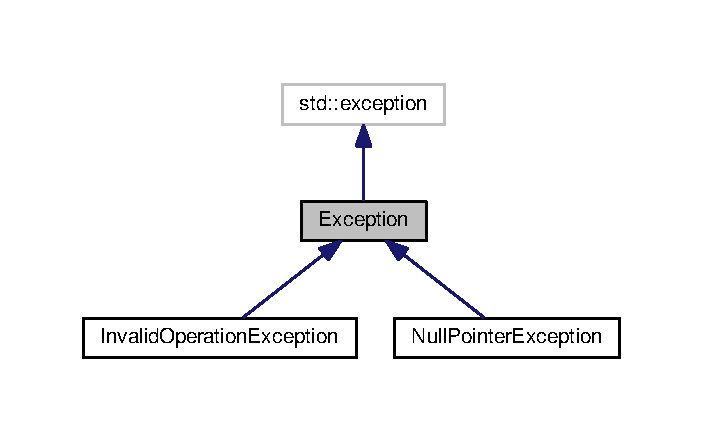
\includegraphics[width=338pt]{classException__inherit__graph}
\end{center}
\end{figure}


Collaboration diagram for Exception\+:\nopagebreak
\begin{figure}[H]
\begin{center}
\leavevmode
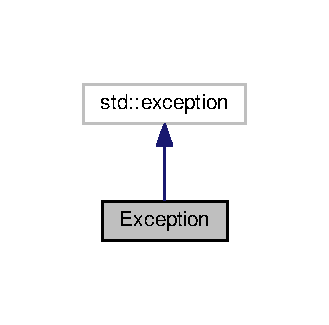
\includegraphics[width=158pt]{classException__coll__graph}
\end{center}
\end{figure}
\subsection*{Public Member Functions}
\begin{Indent}{\bf Constructors/\+Destructor}\par
\begin{DoxyCompactItemize}
\item 
\hyperlink{classException_a3b39c4d55202aea6be3247793e46e2b0}{Exception} (const std\+::string \&msg=\char`\"{}\char`\"{}, const std\+::string \&filename=\char`\"{} \char`\"{}, size\+\_\+t line=0, const std\+::string \&function=\char`\"{} \char`\"{})\hypertarget{classException_a3b39c4d55202aea6be3247793e46e2b0}{}\label{classException_a3b39c4d55202aea6be3247793e46e2b0}

\begin{DoxyCompactList}\small\item\em Constructs exception from message. \end{DoxyCompactList}\item 
\hyperlink{classException_ae0fd52e62283ee92c085d767d0aab736}{Exception} (const \hyperlink{classException}{Exception} \&other)  throw ()\hypertarget{classException_ae0fd52e62283ee92c085d767d0aab736}{}\label{classException_ae0fd52e62283ee92c085d767d0aab736}

\begin{DoxyCompactList}\small\item\em Copy constructor. \end{DoxyCompactList}\item 
\hyperlink{classException}{Exception} \& \hyperlink{classException_a71c844ee3ac32b7656c24386e9ab60a0}{operator=} (const \hyperlink{classException}{Exception} \&other)  throw ()\hypertarget{classException_a71c844ee3ac32b7656c24386e9ab60a0}{}\label{classException_a71c844ee3ac32b7656c24386e9ab60a0}

\begin{DoxyCompactList}\small\item\em Assignment operator. \end{DoxyCompactList}\item 
virtual \hyperlink{classException_ad1ba411de295ef2eeb02ba26284a829a}{$\sim$\+Exception} ()  throw ()\hypertarget{classException_ad1ba411de295ef2eeb02ba26284a829a}{}\label{classException_ad1ba411de295ef2eeb02ba26284a829a}

\begin{DoxyCompactList}\small\item\em Destructor. \end{DoxyCompactList}\end{DoxyCompactItemize}
\end{Indent}
\begin{Indent}{\bf Accessors}\par
\begin{DoxyCompactItemize}
\item 
virtual const char $\ast$ \hyperlink{classException_a78154a31544a609cbd226d32574f52cd}{what} () const   throw ()\hypertarget{classException_a78154a31544a609cbd226d32574f52cd}{}\label{classException_a78154a31544a609cbd226d32574f52cd}

\begin{DoxyCompactList}\small\item\em Access the exception string. \end{DoxyCompactList}\end{DoxyCompactItemize}
\end{Indent}
\subsection*{Protected Attributes}
\begin{Indent}{\bf Protected members}\par
\begin{DoxyCompactItemize}
\item 
std\+::string \hyperlink{classException_a9141b17564f091623cf5a3928e0e0ab3}{m\+Msg}\hypertarget{classException_a9141b17564f091623cf5a3928e0e0ab3}{}\label{classException_a9141b17564f091623cf5a3928e0e0ab3}

\begin{DoxyCompactList}\small\item\em Message in the exception. \end{DoxyCompactList}\item 
std\+::string \hyperlink{classException_a04156475e91fe60dc071c292cf5e2354}{m\+Filename}\hypertarget{classException_a04156475e91fe60dc071c292cf5e2354}{}\label{classException_a04156475e91fe60dc071c292cf5e2354}

\begin{DoxyCompactList}\small\item\em Filename where the exception occurs. \end{DoxyCompactList}\item 
std\+::string \hyperlink{classException_a9eb42c5d2040a0fb75af4d69efa657a1}{m\+Function}\hypertarget{classException_a9eb42c5d2040a0fb75af4d69efa657a1}{}\label{classException_a9eb42c5d2040a0fb75af4d69efa657a1}

\begin{DoxyCompactList}\small\item\em Function where the exception occurs. \end{DoxyCompactList}\item 
size\+\_\+t \hyperlink{classException_a2ece5a599bfb85307da33e61192feddf}{m\+Line}\hypertarget{classException_a2ece5a599bfb85307da33e61192feddf}{}\label{classException_a2ece5a599bfb85307da33e61192feddf}

\begin{DoxyCompactList}\small\item\em Line number where the exception occurs. \end{DoxyCompactList}\item 
std\+::string \hyperlink{classException_a1a8fc6e1adf85832d1dcb253cb5c6329}{m\+Output\+Message}\hypertarget{classException_a1a8fc6e1adf85832d1dcb253cb5c6329}{}\label{classException_a1a8fc6e1adf85832d1dcb253cb5c6329}

\begin{DoxyCompactList}\small\item\em Output message. \end{DoxyCompactList}\end{DoxyCompactItemize}
\end{Indent}


\subsection{Detailed Description}
\hyperlink{classException}{Exception} base class. 

The class \hyperlink{classException}{Exception} represents the base class for all exceptions. 

The documentation for this class was generated from the following file\+:\begin{DoxyCompactItemize}
\item 
/home/tariq/\+Documents/\+M\+A\+T\+L\+A\+B/\+Robust-\/\+View-\/\+Graph-\/\+S\+L\+A\+M/include/\hyperlink{Exception_8h}{Exception.\+h}\end{DoxyCompactItemize}

\hypertarget{classFeatureSelector}{}\section{Feature\+Selector Class Reference}
\label{classFeatureSelector}\index{Feature\+Selector@{Feature\+Selector}}
\subsection*{Public Member Functions}
\begin{DoxyCompactItemize}
\item 
{\bfseries Feature\+Selector} (yarp\+::os\+::\+Resource\+Finder \+\_\+rf)\hypertarget{classFeatureSelector_a363371620000b919b60deb13e00bb743}{}\label{classFeatureSelector_a363371620000b919b60deb13e00bb743}

\item 
bool {\bfseries process} (cv\+::\+Ptr$<$ cv\+::\+Feature2D $>$ \&detector, cv\+::\+Ptr$<$ cv\+::\+Feature2D $>$ \&descriptor, cv\+::\+Ptr$<$ cv\+::\+Descriptor\+Matcher $>$ \&matcher)\hypertarget{classFeatureSelector_a543c2e9e54d6d1d3a6de7db5c19e3763}{}\label{classFeatureSelector_a543c2e9e54d6d1d3a6de7db5c19e3763}

\end{DoxyCompactItemize}
\subsection*{Protected Member Functions}
\begin{DoxyCompactItemize}
\item 
int {\bfseries parse\+Map} (std\+::string value, std\+::map$<$ std\+::string, int $>$ \&m)\hypertarget{classFeatureSelector_a661d1a367c3b88a89ce0efe094baa64a}{}\label{classFeatureSelector_a661d1a367c3b88a89ce0efe094baa64a}

\item 
bool {\bfseries check\+Detector} (std\+::string str)\hypertarget{classFeatureSelector_a037cb04383dd308effd3f7605ac6a3c8}{}\label{classFeatureSelector_a037cb04383dd308effd3f7605ac6a3c8}

\item 
bool {\bfseries check\+Descriptor} (std\+::string str)\hypertarget{classFeatureSelector_a2913a660c607fd69bfdac130c5812ace}{}\label{classFeatureSelector_a2913a660c607fd69bfdac130c5812ace}

\item 
bool {\bfseries check\+Matcher} (std\+::string str, int \+\_\+desc\+ID)\hypertarget{classFeatureSelector_a40d109b2f6774cacb21a96f4dfb13af4}{}\label{classFeatureSelector_a40d109b2f6774cacb21a96f4dfb13af4}

\item 
void {\bfseries switcher} (int det\+ID, int desc\+ID, int match\+ID, cv\+::\+Ptr$<$ cv\+::\+Feature2D $>$ \&detector, cv\+::\+Ptr$<$ cv\+::\+Feature2D $>$ \&descriptor, cv\+::\+Ptr$<$ cv\+::\+Descriptor\+Matcher $>$ \&matcher)\hypertarget{classFeatureSelector_a20d8aa21ec7d99cffde7af05cee5bcbc}{}\label{classFeatureSelector_a20d8aa21ec7d99cffde7af05cee5bcbc}

\item 
int {\bfseries assign\+Method} (std\+::string str)\hypertarget{classFeatureSelector_aaa6c7cbea4869d53b44ef785d78d5063}{}\label{classFeatureSelector_aaa6c7cbea4869d53b44ef785d78d5063}

\end{DoxyCompactItemize}


The documentation for this class was generated from the following files\+:\begin{DoxyCompactItemize}
\item 
/home/tariq/\+Documents/\+M\+A\+T\+L\+A\+B/\+Robust-\/\+View-\/\+Graph-\/\+S\+L\+A\+M/include/featureselector.\+h\item 
/home/tariq/\+Documents/\+M\+A\+T\+L\+A\+B/\+Robust-\/\+View-\/\+Graph-\/\+S\+L\+A\+M/src/featureselector.\+cpp\end{DoxyCompactItemize}

\hypertarget{classGraphOptimiser}{}\section{Graph\+Optimiser Class Reference}
\label{classGraphOptimiser}\index{Graph\+Optimiser@{Graph\+Optimiser}}
\subsection*{Public Member Functions}
\begin{DoxyCompactItemize}
\item 
void {\bfseries initialise\+\_\+a\+\_\+constraint} (const std\+::vector$<$ double $>$ \&edge, const std\+::vector$<$ double $>$ \&z, const std\+::vector$<$ double $>$ \&R)\hypertarget{classGraphOptimiser_ab58070fd7b8196c9e1bd7e41d2df0eca}{}\label{classGraphOptimiser_ab58070fd7b8196c9e1bd7e41d2df0eca}

\item 
void {\bfseries compute\+\_\+gate} (double $\ast$gate, double $\ast$x, double $\ast$s, double $\ast$xs, long unsigned int ncols)\hypertarget{classGraphOptimiser_a7be156050f369b6354a95b36ff12809c}{}\label{classGraphOptimiser_a7be156050f369b6354a95b36ff12809c}

\end{DoxyCompactItemize}


The documentation for this class was generated from the following files\+:\begin{DoxyCompactItemize}
\item 
/home/tariq/\+Documents/\+M\+A\+T\+L\+A\+B/\+Robust-\/\+View-\/\+Graph-\/\+S\+L\+A\+M/include/Graph\+Optimiser.\+h\item 
/home/tariq/\+Documents/\+M\+A\+T\+L\+A\+B/\+Robust-\/\+View-\/\+Graph-\/\+S\+L\+A\+M/src/Graph\+Optimiser.\+cpp\end{DoxyCompactItemize}

\hypertarget{classImage}{}\section{Image Class Reference}
\label{classImage}\index{Image@{Image}}


Collaboration diagram for Image\+:\nopagebreak
\begin{figure}[H]
\begin{center}
\leavevmode
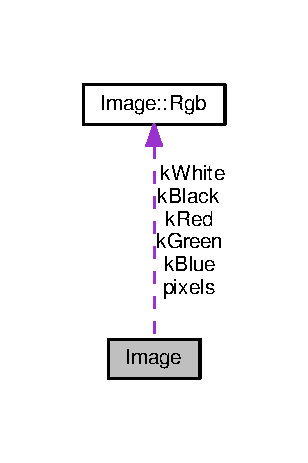
\includegraphics[width=148pt]{classImage__coll__graph}
\end{center}
\end{figure}
\subsection*{Classes}
\begin{DoxyCompactItemize}
\item 
struct \hyperlink{structImage_1_1Rgb}{Rgb}
\end{DoxyCompactItemize}
\subsection*{Public Member Functions}
\begin{DoxyCompactItemize}
\item 
{\bfseries Image} (const unsigned int \&\+\_\+w, const unsigned int \&\+\_\+h, const \hyperlink{structImage_1_1Rgb}{Rgb} \&c=k\+Black)\hypertarget{classImage_a0ad0eb194da218c3402a187c1d339adb}{}\label{classImage_a0ad0eb194da218c3402a187c1d339adb}

\item 
const \hyperlink{structImage_1_1Rgb}{Rgb} \& {\bfseries operator\mbox{[}$\,$\mbox{]}} (const unsigned int \&i) const \hypertarget{classImage_a86c78da799bb20ff07924de0070f7909}{}\label{classImage_a86c78da799bb20ff07924de0070f7909}

\item 
\hyperlink{structImage_1_1Rgb}{Rgb} \& {\bfseries operator\mbox{[}$\,$\mbox{]}} (const unsigned int \&i)\hypertarget{classImage_a81577616707e17b4b1fdee5eb49151c8}{}\label{classImage_a81577616707e17b4b1fdee5eb49151c8}

\end{DoxyCompactItemize}
\subsection*{Public Attributes}
\begin{DoxyCompactItemize}
\item 
unsigned int {\bfseries w}\hypertarget{classImage_ab543158db8f1e052304cf19bd16039fd}{}\label{classImage_ab543158db8f1e052304cf19bd16039fd}

\item 
unsigned int {\bfseries h}\hypertarget{classImage_a3df6171bcc6186a4598cba8062a63f3b}{}\label{classImage_a3df6171bcc6186a4598cba8062a63f3b}

\item 
\hyperlink{structImage_1_1Rgb}{Rgb} $\ast$ {\bfseries pixels}\hypertarget{classImage_adb981556f5bcd694863db42caecda726}{}\label{classImage_adb981556f5bcd694863db42caecda726}

\end{DoxyCompactItemize}
\subsection*{Static Public Attributes}
\begin{DoxyCompactItemize}
\item 
static const \hyperlink{structImage_1_1Rgb}{Rgb} {\bfseries k\+Black} = \hyperlink{structImage_1_1Rgb}{Image\+::\+Rgb}(0)\hypertarget{classImage_a3af1a2f15969cb91d7855dde1b1636fc}{}\label{classImage_a3af1a2f15969cb91d7855dde1b1636fc}

\item 
static const \hyperlink{structImage_1_1Rgb}{Rgb} {\bfseries k\+White} = \hyperlink{structImage_1_1Rgb}{Image\+::\+Rgb}(1)\hypertarget{classImage_a0d566dca18997bf5476b44533fd6f47e}{}\label{classImage_a0d566dca18997bf5476b44533fd6f47e}

\item 
static const \hyperlink{structImage_1_1Rgb}{Rgb} {\bfseries k\+Red} = \hyperlink{structImage_1_1Rgb}{Image\+::\+Rgb}(1,0,0)\hypertarget{classImage_a608a338f74b08734f178564054a0795a}{}\label{classImage_a608a338f74b08734f178564054a0795a}

\item 
static const \hyperlink{structImage_1_1Rgb}{Rgb} {\bfseries k\+Green} = \hyperlink{structImage_1_1Rgb}{Image\+::\+Rgb}(0,1,0)\hypertarget{classImage_a3fdac82511a82f222766220d4a9add8e}{}\label{classImage_a3fdac82511a82f222766220d4a9add8e}

\item 
static const \hyperlink{structImage_1_1Rgb}{Rgb} {\bfseries k\+Blue} = \hyperlink{structImage_1_1Rgb}{Image\+::\+Rgb}(0,0,1)\hypertarget{classImage_a4da8b48b3fc304a8e17f591e58b44afb}{}\label{classImage_a4da8b48b3fc304a8e17f591e58b44afb}

\end{DoxyCompactItemize}


The documentation for this class was generated from the following file\+:\begin{DoxyCompactItemize}
\item 
/home/tariq/\+Documents/\+M\+A\+T\+L\+A\+B/\+Robust-\/\+View-\/\+Graph-\/\+S\+L\+A\+M/include/Image.\+h\end{DoxyCompactItemize}

\hypertarget{classInvalidOperationException}{}\section{Invalid\+Operation\+Exception Class Reference}
\label{classInvalidOperationException}\index{Invalid\+Operation\+Exception@{Invalid\+Operation\+Exception}}


Invalid operation exception.  




{\ttfamily \#include $<$Invalid\+Operation\+Exception.\+h$>$}



Inheritance diagram for Invalid\+Operation\+Exception\+:\nopagebreak
\begin{figure}[H]
\begin{center}
\leavevmode
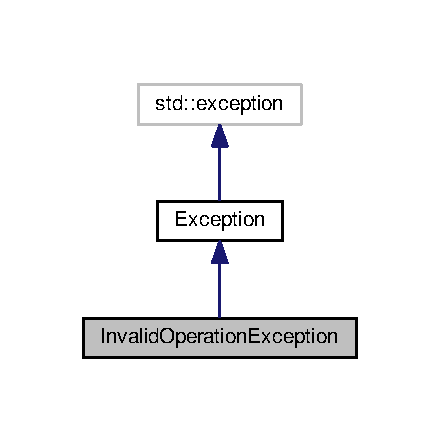
\includegraphics[width=211pt]{classInvalidOperationException__inherit__graph}
\end{center}
\end{figure}


Collaboration diagram for Invalid\+Operation\+Exception\+:\nopagebreak
\begin{figure}[H]
\begin{center}
\leavevmode
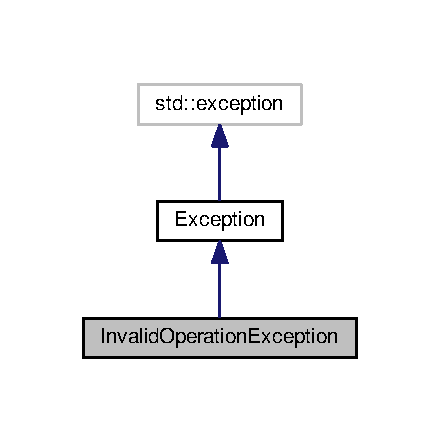
\includegraphics[width=211pt]{classInvalidOperationException__coll__graph}
\end{center}
\end{figure}
\subsection*{Public Member Functions}
\begin{Indent}{\bf Constructors/\+Destructor}\par
\begin{DoxyCompactItemize}
\item 
\hyperlink{classInvalidOperationException_affce63f9604d0c392946e62eef9917c0}{Invalid\+Operation\+Exception} (const std\+::string \&msg=\char`\"{}\char`\"{}, const std\+::string \&filename=\char`\"{} \char`\"{}, size\+\_\+t line=0, const std\+::string \&function=\char`\"{} \char`\"{})\hypertarget{classInvalidOperationException_affce63f9604d0c392946e62eef9917c0}{}\label{classInvalidOperationException_affce63f9604d0c392946e62eef9917c0}

\begin{DoxyCompactList}\small\item\em Constructs exception from message. \end{DoxyCompactList}\item 
\hyperlink{classInvalidOperationException_ad18f00b8fe7516ab6b8c2028376c0805}{Invalid\+Operation\+Exception} (const \hyperlink{classInvalidOperationException}{Invalid\+Operation\+Exception} \&other)  throw ()\hypertarget{classInvalidOperationException_ad18f00b8fe7516ab6b8c2028376c0805}{}\label{classInvalidOperationException_ad18f00b8fe7516ab6b8c2028376c0805}

\begin{DoxyCompactList}\small\item\em Copy constructor. \end{DoxyCompactList}\item 
\hyperlink{classInvalidOperationException}{Invalid\+Operation\+Exception} \& \hyperlink{classInvalidOperationException_a482ed8869e13ab5db6f5ee67abf05112}{operator=} (const \hyperlink{classInvalidOperationException}{Invalid\+Operation\+Exception} \&other)  throw ()\hypertarget{classInvalidOperationException_a482ed8869e13ab5db6f5ee67abf05112}{}\label{classInvalidOperationException_a482ed8869e13ab5db6f5ee67abf05112}

\begin{DoxyCompactList}\small\item\em Assignment operator. \end{DoxyCompactList}\item 
virtual \hyperlink{classInvalidOperationException_a0047dfc9b947476091ac3ea8bcd8cedf}{$\sim$\+Invalid\+Operation\+Exception} ()  throw ()\hypertarget{classInvalidOperationException_a0047dfc9b947476091ac3ea8bcd8cedf}{}\label{classInvalidOperationException_a0047dfc9b947476091ac3ea8bcd8cedf}

\begin{DoxyCompactList}\small\item\em Destructor. \end{DoxyCompactList}\end{DoxyCompactItemize}
\end{Indent}
\subsection*{Additional Inherited Members}


\subsection{Detailed Description}
Invalid operation exception. 

The class \hyperlink{classInvalidOperationException}{Invalid\+Operation\+Exception} represents invalid operations exceptions. 

The documentation for this class was generated from the following file\+:\begin{DoxyCompactItemize}
\item 
/home/tariq/\+Documents/\+M\+A\+T\+L\+A\+B/\+Robust-\/\+View-\/\+Graph-\/\+S\+L\+A\+M/include/\hyperlink{InvalidOperationException_8h}{Invalid\+Operation\+Exception.\+h}\end{DoxyCompactItemize}

\hypertarget{classNullPointerException}{}\section{Null\+Pointer\+Exception Class Reference}
\label{classNullPointerException}\index{Null\+Pointer\+Exception@{Null\+Pointer\+Exception}}


Null pointer exception.  




{\ttfamily \#include $<$Null\+Pointer\+Exception.\+h$>$}



Inheritance diagram for Null\+Pointer\+Exception\+:\nopagebreak
\begin{figure}[H]
\begin{center}
\leavevmode
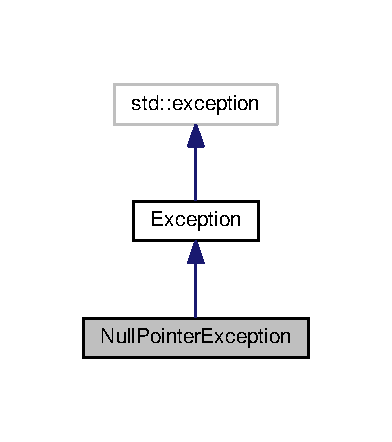
\includegraphics[width=188pt]{classNullPointerException__inherit__graph}
\end{center}
\end{figure}


Collaboration diagram for Null\+Pointer\+Exception\+:\nopagebreak
\begin{figure}[H]
\begin{center}
\leavevmode
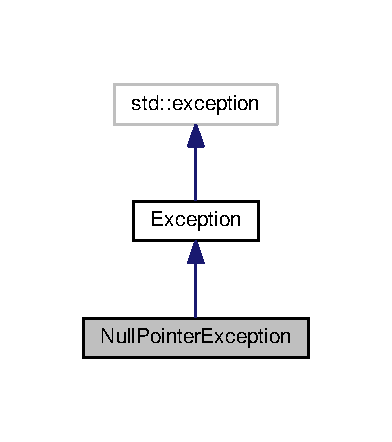
\includegraphics[width=188pt]{classNullPointerException__coll__graph}
\end{center}
\end{figure}
\subsection*{Public Member Functions}
\begin{Indent}{\bf Constructors/\+Destructor}\par
\begin{DoxyCompactItemize}
\item 
\hyperlink{classNullPointerException_ac582ad9b8b3b1a7e5086eddc51f45341}{Null\+Pointer\+Exception} (const std\+::string \&name=\char`\"{}\char`\"{}, const std\+::string \&filename=\char`\"{} \char`\"{}, size\+\_\+t line=0, const std\+::string \&function=\char`\"{} \char`\"{})\hypertarget{classNullPointerException_ac582ad9b8b3b1a7e5086eddc51f45341}{}\label{classNullPointerException_ac582ad9b8b3b1a7e5086eddc51f45341}

\begin{DoxyCompactList}\small\item\em Constructs exception from message. \end{DoxyCompactList}\item 
\hyperlink{classNullPointerException_a7ec1e957cb13533582034e08971ce739}{Null\+Pointer\+Exception} (const \hyperlink{classNullPointerException}{Null\+Pointer\+Exception} \&other)  throw ()\hypertarget{classNullPointerException_a7ec1e957cb13533582034e08971ce739}{}\label{classNullPointerException_a7ec1e957cb13533582034e08971ce739}

\begin{DoxyCompactList}\small\item\em Copy constructor. \end{DoxyCompactList}\item 
\hyperlink{classNullPointerException}{Null\+Pointer\+Exception} \& \hyperlink{classNullPointerException_a77345c84b84d5d79be16b3c987a54155}{operator=} (const \hyperlink{classNullPointerException}{Null\+Pointer\+Exception} \&other)  throw ()\hypertarget{classNullPointerException_a77345c84b84d5d79be16b3c987a54155}{}\label{classNullPointerException_a77345c84b84d5d79be16b3c987a54155}

\begin{DoxyCompactList}\small\item\em Assignment operator. \end{DoxyCompactList}\item 
virtual \hyperlink{classNullPointerException_a94d055526c67a34ba55d7bf8bf108adb}{$\sim$\+Null\+Pointer\+Exception} ()  throw ()\hypertarget{classNullPointerException_a94d055526c67a34ba55d7bf8bf108adb}{}\label{classNullPointerException_a94d055526c67a34ba55d7bf8bf108adb}

\begin{DoxyCompactList}\small\item\em Destructor. \end{DoxyCompactList}\end{DoxyCompactItemize}
\end{Indent}
\subsection*{Additional Inherited Members}


\subsection{Detailed Description}
Null pointer exception. 

The class \hyperlink{classNullPointerException}{Null\+Pointer\+Exception} represents null pointer exceptions. 

The documentation for this class was generated from the following file\+:\begin{DoxyCompactItemize}
\item 
/home/tariq/\+Documents/\+M\+A\+T\+L\+A\+B/\+Robust-\/\+View-\/\+Graph-\/\+S\+L\+A\+M/include/\hyperlink{NullPointerException_8h}{Null\+Pointer\+Exception.\+h}\end{DoxyCompactItemize}

\hypertarget{structPair}{}\section{Pair Struct Reference}
\label{structPair}\index{Pair@{Pair}}
\subsection*{Public Attributes}
\begin{DoxyCompactItemize}
\item 
int {\bfseries k1}\hypertarget{structPair_a845d12e75b8a55691f3bb6f48b659968}{}\label{structPair_a845d12e75b8a55691f3bb6f48b659968}

\item 
int {\bfseries k2}\hypertarget{structPair_a663b93b2a769419e7d325fc13a69be55}{}\label{structPair_a663b93b2a769419e7d325fc13a69be55}

\item 
double {\bfseries score}\hypertarget{structPair_aa8d11c69d77a839c11ff2668360a1ce7}{}\label{structPair_aa8d11c69d77a839c11ff2668360a1ce7}

\end{DoxyCompactItemize}


The documentation for this struct was generated from the following file\+:\begin{DoxyCompactItemize}
\item 
/home/tariq/\+Documents/\+M\+A\+T\+L\+A\+B/\+Robust-\/\+View-\/\+Graph-\/\+S\+L\+A\+M/src/V\+L\+Feat.\+cpp\end{DoxyCompactItemize}

\hypertarget{structTracker_1_1point__2d}{}\section{Tracker\+:\+:point\+\_\+2d Struct Reference}
\label{structTracker_1_1point__2d}\index{Tracker\+::point\+\_\+2d@{Tracker\+::point\+\_\+2d}}
\subsection*{Public Member Functions}
\begin{DoxyCompactItemize}
\item 
{\bfseries point\+\_\+2d} (std\+::vector$<$ double $>$ \&a, std\+::vector$<$ double $>$ \&b, std\+::vector$<$ int $>$ \&c, int d)\hypertarget{structTracker_1_1point__2d_ab452d62cdc5f07e21dd3c1343d1f5951}{}\label{structTracker_1_1point__2d_ab452d62cdc5f07e21dd3c1343d1f5951}

\end{DoxyCompactItemize}
\subsection*{Public Attributes}
\begin{DoxyCompactItemize}
\item 
const std\+::vector$<$ double $>$ {\bfseries x}\hypertarget{structTracker_1_1point__2d_a7b5555f1e9d4459cd19b69190e68d4c4}{}\label{structTracker_1_1point__2d_a7b5555f1e9d4459cd19b69190e68d4c4}

\item 
const std\+::vector$<$ double $>$ {\bfseries y}\hypertarget{structTracker_1_1point__2d_aa226e7fc9461a164dc12e4f5d85f531a}{}\label{structTracker_1_1point__2d_aa226e7fc9461a164dc12e4f5d85f531a}

\item 
const std\+::vector$<$ int $>$ {\bfseries status}\hypertarget{structTracker_1_1point__2d_a2f457ea97e5cc7e4a8ba1aeffbad15ac}{}\label{structTracker_1_1point__2d_a2f457ea97e5cc7e4a8ba1aeffbad15ac}

\item 
int {\bfseries camera}\hypertarget{structTracker_1_1point__2d_a095f7164767f1e4f17a60c3856ddd75a}{}\label{structTracker_1_1point__2d_a095f7164767f1e4f17a60c3856ddd75a}

\item 
int {\bfseries npts}\hypertarget{structTracker_1_1point__2d_a891f773f43c2079df404f57aa8a9f5fb}{}\label{structTracker_1_1point__2d_a891f773f43c2079df404f57aa8a9f5fb}

\end{DoxyCompactItemize}


The documentation for this struct was generated from the following file\+:\begin{DoxyCompactItemize}
\item 
/home/tariq/\+Documents/\+M\+A\+T\+L\+A\+B/\+Robust-\/\+View-\/\+Graph-\/\+S\+L\+A\+M/include/Tracker.\+h\end{DoxyCompactItemize}

\hypertarget{classPolyMatrix}{}\section{Poly\+Matrix Class Reference}
\label{classPolyMatrix}\index{Poly\+Matrix@{Poly\+Matrix}}
\subsection*{Public Member Functions}
\begin{DoxyCompactItemize}
\item 
{\bfseries Poly\+Matrix} (int rows, int cols)\hypertarget{classPolyMatrix_ac93ab07429acd1c7121bbe28f27fc7d1}{}\label{classPolyMatrix_ac93ab07429acd1c7121bbe28f27fc7d1}

\item 
\hyperlink{classPolynomial}{Polynomial} \& {\bfseries operator()} (int row, int col)\hypertarget{classPolyMatrix_aaa9b3c90712f4c2164b66f9651b5b3f8}{}\label{classPolyMatrix_aaa9b3c90712f4c2164b66f9651b5b3f8}

\item 
void {\bfseries Eval} (double x, double $\ast$ret)\hypertarget{classPolyMatrix_a0ca0aef742c645d0a4939d7c57fffdaf}{}\label{classPolyMatrix_a0ca0aef742c645d0a4939d7c57fffdaf}

\end{DoxyCompactItemize}
\subsection*{Public Attributes}
\begin{DoxyCompactItemize}
\item 
int {\bfseries m\+\_\+rows}\hypertarget{classPolyMatrix_ad712044158b69bcfb7b0ddc00833e7af}{}\label{classPolyMatrix_ad712044158b69bcfb7b0ddc00833e7af}

\item 
int {\bfseries m\+\_\+cols}\hypertarget{classPolyMatrix_a5cca7b71143efc040cd380de4d0defce}{}\label{classPolyMatrix_a5cca7b71143efc040cd380de4d0defce}

\item 
std\+::vector$<$ std\+::vector$<$ \hyperlink{classPolynomial}{Polynomial} $>$ $>$ {\bfseries m\+\_\+data}\hypertarget{classPolyMatrix_a4290f16939adce36dfc4dbf0cd3ca3bc}{}\label{classPolyMatrix_a4290f16939adce36dfc4dbf0cd3ca3bc}

\end{DoxyCompactItemize}
\subsection*{Friends}
\begin{DoxyCompactItemize}
\item 
std\+::ostream \& {\bfseries operator$<$$<$} (std\+::ostream \&os, const \hyperlink{classPolyMatrix}{Poly\+Matrix} \&p)\hypertarget{classPolyMatrix_a972de29f696a52bdd12c8c3e8499501b}{}\label{classPolyMatrix_a972de29f696a52bdd12c8c3e8499501b}

\end{DoxyCompactItemize}


The documentation for this class was generated from the following file\+:\begin{DoxyCompactItemize}
\item 
/home/tariq/\+Documents/\+M\+A\+T\+L\+A\+B/\+Robust-\/\+View-\/\+Graph-\/\+S\+L\+A\+M/include/Polynomial.\+h\end{DoxyCompactItemize}

\hypertarget{classPolynomial}{}\section{Polynomial Class Reference}
\label{classPolynomial}\index{Polynomial@{Polynomial}}
\subsection*{Public Member Functions}
\begin{DoxyCompactItemize}
\item 
double \& {\bfseries operator\mbox{[}$\,$\mbox{]}} (int power)\hypertarget{classPolynomial_a8159721fa561bf68f6ad0c61e1ab28c4}{}\label{classPolynomial_a8159721fa561bf68f6ad0c61e1ab28c4}

\item 
double {\bfseries operator\mbox{[}$\,$\mbox{]}} (int power) const \hypertarget{classPolynomial_a4bd5fb1ace3d3ad09d9fbde9ede70cad}{}\label{classPolynomial_a4bd5fb1ace3d3ad09d9fbde9ede70cad}

\item 
double {\bfseries Eval} (double x)\hypertarget{classPolynomial_ae29c3326a10502032cdffcaccec7055f}{}\label{classPolynomial_ae29c3326a10502032cdffcaccec7055f}

\item 
\hyperlink{classPolynomial}{Polynomial} {\bfseries operator$\ast$} (const double val) const \hypertarget{classPolynomial_a72f47976238507e269fc3499ddb8fd37}{}\label{classPolynomial_a72f47976238507e269fc3499ddb8fd37}

\item 
\hyperlink{classPolynomial}{Polynomial} \& {\bfseries operator$\ast$=} (const double val)\hypertarget{classPolynomial_a168553118ab5269e1597f9b33d8d70a1}{}\label{classPolynomial_a168553118ab5269e1597f9b33d8d70a1}

\item 
\hyperlink{classPolynomial}{Polynomial} {\bfseries operator$\ast$} (const \hyperlink{classPolynomial}{Polynomial} \&rhs) const \hypertarget{classPolynomial_a1e00f25b4de1d335f437749c7bd93ac9}{}\label{classPolynomial_a1e00f25b4de1d335f437749c7bd93ac9}

\item 
\hyperlink{classPolynomial}{Polynomial} \& {\bfseries operator$\ast$=} (const \hyperlink{classPolynomial}{Polynomial} \&rhs)\hypertarget{classPolynomial_a2fe2da05d52f0c8866b9b55130e48f0e}{}\label{classPolynomial_a2fe2da05d52f0c8866b9b55130e48f0e}

\item 
\hyperlink{classPolynomial}{Polynomial} {\bfseries operator+} (const \hyperlink{classPolynomial}{Polynomial} \&rhs) const \hypertarget{classPolynomial_a42b8d27c68921d613367826990644e70}{}\label{classPolynomial_a42b8d27c68921d613367826990644e70}

\item 
\hyperlink{classPolynomial}{Polynomial} \& {\bfseries operator+=} (const \hyperlink{classPolynomial}{Polynomial} \&rhs)\hypertarget{classPolynomial_a0309358e97b5a50b2fe13f5242d68f38}{}\label{classPolynomial_a0309358e97b5a50b2fe13f5242d68f38}

\item 
\hyperlink{classPolynomial}{Polynomial} {\bfseries operator-\/} (const \hyperlink{classPolynomial}{Polynomial} \&rhs) const \hypertarget{classPolynomial_acff0b8a8c385f43f9d57c80ee925d858}{}\label{classPolynomial_acff0b8a8c385f43f9d57c80ee925d858}

\item 
\hyperlink{classPolynomial}{Polynomial} \& {\bfseries operator-\/=} (const \hyperlink{classPolynomial}{Polynomial} \&rhs)\hypertarget{classPolynomial_a19e1abe808b7cc063edef7249c2b2bbf}{}\label{classPolynomial_a19e1abe808b7cc063edef7249c2b2bbf}

\end{DoxyCompactItemize}
\subsection*{Public Attributes}
\begin{DoxyCompactItemize}
\item 
std\+::vector$<$ double $>$ {\bfseries m\+\_\+coeffs}\hypertarget{classPolynomial_a67e77ed96a49e4f16be5c6be158e7e24}{}\label{classPolynomial_a67e77ed96a49e4f16be5c6be158e7e24}

\end{DoxyCompactItemize}
\subsection*{Friends}
\begin{DoxyCompactItemize}
\item 
std\+::ostream \& {\bfseries operator$<$$<$} (std\+::ostream \&os, const \hyperlink{classPolynomial}{Polynomial} \&p)\hypertarget{classPolynomial_af1fdf53b29100b084772816cb9ecc8ac}{}\label{classPolynomial_af1fdf53b29100b084772816cb9ecc8ac}

\end{DoxyCompactItemize}


The documentation for this class was generated from the following file\+:\begin{DoxyCompactItemize}
\item 
/home/tariq/\+Documents/\+M\+A\+T\+L\+A\+B/\+Robust-\/\+View-\/\+Graph-\/\+S\+L\+A\+M/include/Polynomial.\+h\end{DoxyCompactItemize}

\hypertarget{structPwgOptimiser_1_1pulled__constraint}{}\section{Pwg\+Optimiser\+:\+:pulled\+\_\+constraint Struct Reference}
\label{structPwgOptimiser_1_1pulled__constraint}\index{Pwg\+Optimiser\+::pulled\+\_\+constraint@{Pwg\+Optimiser\+::pulled\+\_\+constraint}}
\subsection*{Public Member Functions}
\begin{DoxyCompactItemize}
\item 
{\bfseries pulled\+\_\+constraint} (const constraint C)\hypertarget{structPwgOptimiser_1_1pulled__constraint_a73c3accc55b8ff93376dbcf8e8ab12a2}{}\label{structPwgOptimiser_1_1pulled__constraint_a73c3accc55b8ff93376dbcf8e8ab12a2}

\end{DoxyCompactItemize}
\subsection*{Public Attributes}
\begin{DoxyCompactItemize}
\item 
const int {\bfseries cam}\hypertarget{structPwgOptimiser_1_1pulled__constraint_a6baab11c5c10c4411ba07d4d5397f973}{}\label{structPwgOptimiser_1_1pulled__constraint_a6baab11c5c10c4411ba07d4d5397f973}

\item 
const int {\bfseries kpt}\hypertarget{structPwgOptimiser_1_1pulled__constraint_a0caa4348b0544a74d0231c2be83a9324}{}\label{structPwgOptimiser_1_1pulled__constraint_a0caa4348b0544a74d0231c2be83a9324}

\item 
const std\+::vector$<$ double $>$ {\bfseries p1}\hypertarget{structPwgOptimiser_1_1pulled__constraint_ad755df2c3eea4f84987883f41b62eede}{}\label{structPwgOptimiser_1_1pulled__constraint_ad755df2c3eea4f84987883f41b62eede}

\item 
const std\+::vector$<$ double $>$ {\bfseries z}\hypertarget{structPwgOptimiser_1_1pulled__constraint_ab64d97f866b4771b20c2e57ebfe644e2}{}\label{structPwgOptimiser_1_1pulled__constraint_ab64d97f866b4771b20c2e57ebfe644e2}

\item 
const std\+::vector$<$ double $>$ {\bfseries R}\hypertarget{structPwgOptimiser_1_1pulled__constraint_a25ea6d42c540cb5667e5691082c0a1ae}{}\label{structPwgOptimiser_1_1pulled__constraint_a25ea6d42c540cb5667e5691082c0a1ae}

\item 
const Eigen\+::\+Matrix\+Xd {\bfseries Y}\hypertarget{structPwgOptimiser_1_1pulled__constraint_a9a2792b99e9f01d3aa88d0244fa17243}{}\label{structPwgOptimiser_1_1pulled__constraint_a9a2792b99e9f01d3aa88d0244fa17243}

\item 
const Eigen\+::\+Vector\+Xd {\bfseries y}\hypertarget{structPwgOptimiser_1_1pulled__constraint_ab5c4120cd329a9a63c86020a24f736bd}{}\label{structPwgOptimiser_1_1pulled__constraint_ab5c4120cd329a9a63c86020a24f736bd}

\end{DoxyCompactItemize}


The documentation for this struct was generated from the following file\+:\begin{DoxyCompactItemize}
\item 
/home/tariq/\+Documents/\+M\+A\+T\+L\+A\+B/\+Robust-\/\+View-\/\+Graph-\/\+S\+L\+A\+M/include/\hyperlink{PwgOptimiser_8h}{Pwg\+Optimiser.\+h}\end{DoxyCompactItemize}

\hypertarget{classPwgOptimiser}{}\section{Pwg\+Optimiser Class Reference}
\label{classPwgOptimiser}\index{Pwg\+Optimiser@{Pwg\+Optimiser}}
\subsection*{Classes}
\begin{DoxyCompactItemize}
\item 
struct \hyperlink{structPwgOptimiser_1_1pulled__constraint}{pulled\+\_\+constraint}
\end{DoxyCompactItemize}
\subsection*{Public Member Functions}
\begin{DoxyCompactItemize}
\item 
{\bfseries Pwg\+Optimiser} (int M, int N)\hypertarget{classPwgOptimiser_ab082a4335ae1d71677b4098a3ca6e94b}{}\label{classPwgOptimiser_ab082a4335ae1d71677b4098a3ca6e94b}

\item 
void {\bfseries set\+\_\+information\+\_\+matrix\+\_\+and\+\_\+vector} (Eigen\+::\+Vector\+Xd \&yin, Eigen\+::\+Sparse\+Matrix$<$ double $>$ \&Yin)\hypertarget{classPwgOptimiser_a00fef5371d6840b4c3443ca7daf62672}{}\label{classPwgOptimiser_a00fef5371d6840b4c3443ca7daf62672}

\item 
void {\bfseries get\+\_\+information\+\_\+matrix\+\_\+and\+\_\+vector} (Eigen\+::\+Vector\+Xd \&yout, Eigen\+::\+Sparse\+Matrix$<$ double $>$ \&Yout)\hypertarget{classPwgOptimiser_a210b49d192ca7d98fadb2fa495d07212}{}\label{classPwgOptimiser_a210b49d192ca7d98fadb2fa495d07212}

\item 
void {\bfseries get\+\_\+switch\+\_\+vector} (int $\ast$sw)\hypertarget{classPwgOptimiser_a7bc7c631a1c763a5d1f8896641ca4928}{}\label{classPwgOptimiser_a7bc7c631a1c763a5d1f8896641ca4928}

\item 
void {\bfseries initialise\+\_\+a\+\_\+constraint} (const int \&cam, const int \&kpt, const std\+::vector$<$ double $>$ \&p1, const std\+::vector$<$ double $>$ \&z, const std\+::vector$<$ double $>$ \&R, Eigen\+::\+Matrix\+Xd Y, Eigen\+::\+Vector\+Xd y, const int \&sw)\hypertarget{classPwgOptimiser_a8d775b7dcc5930aa9a0f318e5d1753c2}{}\label{classPwgOptimiser_a8d775b7dcc5930aa9a0f318e5d1753c2}

\item 
void {\bfseries generate\+\_\+constraints\+\_\+info\+\_\+\+Mviews} (const double $\ast$xs)\hypertarget{classPwgOptimiser_aa7755f3adb3807a1a0c4f2aca738e71c}{}\label{classPwgOptimiser_aa7755f3adb3807a1a0c4f2aca738e71c}

\item 
void {\bfseries optimise\+\_\+constraints\+\_\+image\+\_\+inverse\+\_\+depth\+\_\+\+Mviews} (const double $\ast$xs)\hypertarget{classPwgOptimiser_acb4d7544d9e43b0fe51a7c9ec7f1ee1a}{}\label{classPwgOptimiser_acb4d7544d9e43b0fe51a7c9ec7f1ee1a}

\item 
void {\bfseries pull\+\_\+constraints\+\_\+\+Mviews} (std\+::vector$<$ \hyperlink{structPwgOptimiser_1_1pulled__constraint}{pulled\+\_\+constraint} $>$ \&C)\hypertarget{classPwgOptimiser_ac4df16773850e8c9d58a6f5c0a178197}{}\label{classPwgOptimiser_ac4df16773850e8c9d58a6f5c0a178197}

\end{DoxyCompactItemize}
\subsection*{Public Attributes}
\begin{DoxyCompactItemize}
\item 
Eigen\+::\+Sparse\+Matrix$<$ double $>$ {\bfseries Phat}\hypertarget{classPwgOptimiser_a4cae98998f37bc2806cfd8718b8c01cf}{}\label{classPwgOptimiser_a4cae98998f37bc2806cfd8718b8c01cf}

\item 
Eigen\+::\+Vector\+Xd {\bfseries xhat}\hypertarget{classPwgOptimiser_afb15930580a6bec1b31dd986120c825a}{}\label{classPwgOptimiser_afb15930580a6bec1b31dd986120c825a}

\end{DoxyCompactItemize}
\subsection*{Friends}
\begin{DoxyCompactItemize}
\item 
void {\bfseries mex\+Function} (int nlhs, mx\+Array $\ast$plhs\mbox{[}$\,$\mbox{]}, int nrhs, const mx\+Array $\ast$prhs\mbox{[}$\,$\mbox{]})\hypertarget{classPwgOptimiser_a6a215cbfde54f82a3ce599228fc3fce5}{}\label{classPwgOptimiser_a6a215cbfde54f82a3ce599228fc3fce5}

\end{DoxyCompactItemize}


The documentation for this class was generated from the following files\+:\begin{DoxyCompactItemize}
\item 
/home/tariq/\+Documents/\+M\+A\+T\+L\+A\+B/\+Robust-\/\+View-\/\+Graph-\/\+S\+L\+A\+M/include/\hyperlink{PwgOptimiser_8h}{Pwg\+Optimiser.\+h}\item 
/home/tariq/\+Documents/\+M\+A\+T\+L\+A\+B/\+Robust-\/\+View-\/\+Graph-\/\+S\+L\+A\+M/src/Pwg\+Optimiser.\+cpp\end{DoxyCompactItemize}

\hypertarget{classRecoverMoments}{}\section{Recover\+Moments Class Reference}
\label{classRecoverMoments}\index{Recover\+Moments@{Recover\+Moments}}
\subsection*{Public Member Functions}
\begin{DoxyCompactItemize}
\item 
{\bfseries Recover\+Moments} (const Eigen\+::\+Sparse\+Matrix$<$ double $>$ \&A, const Eigen\+::\+Vector\+Xd \&b)\hypertarget{classRecoverMoments_a8653cd56de0d2b208428d8d93e37431c}{}\label{classRecoverMoments_a8653cd56de0d2b208428d8d93e37431c}

\end{DoxyCompactItemize}
\subsection*{Public Attributes}
\begin{DoxyCompactItemize}
\item 
Eigen\+::\+Sparse\+Matrix$<$ double $>$ {\bfseries P}\hypertarget{classRecoverMoments_a3e1c991fafc11e3320b314b96e42e81a}{}\label{classRecoverMoments_a3e1c991fafc11e3320b314b96e42e81a}

\item 
Eigen\+::\+Vector\+Xd {\bfseries x}\hypertarget{classRecoverMoments_a7d791f3d785a9bbb47dfce68e100e481}{}\label{classRecoverMoments_a7d791f3d785a9bbb47dfce68e100e481}

\end{DoxyCompactItemize}


The documentation for this class was generated from the following files\+:\begin{DoxyCompactItemize}
\item 
/home/tariq/\+Documents/\+M\+A\+T\+L\+A\+B/\+Robust-\/\+View-\/\+Graph-\/\+S\+L\+A\+M/include/Recover\+Moments.\+h\item 
/home/tariq/\+Documents/\+M\+A\+T\+L\+A\+B/\+Robust-\/\+View-\/\+Graph-\/\+S\+L\+A\+M/src/Recover\+Moments.\+cpp\end{DoxyCompactItemize}

\hypertarget{structImage_1_1Rgb}{}\section{Image\+:\+:Rgb Struct Reference}
\label{structImage_1_1Rgb}\index{Image\+::\+Rgb@{Image\+::\+Rgb}}
\subsection*{Public Member Functions}
\begin{DoxyCompactItemize}
\item 
{\bfseries Rgb} (float c)\hypertarget{structImage_1_1Rgb_a764740af5f1baa9556e9cad743ed58c0}{}\label{structImage_1_1Rgb_a764740af5f1baa9556e9cad743ed58c0}

\item 
{\bfseries Rgb} (float \+\_\+r, float \+\_\+g, float \+\_\+b)\hypertarget{structImage_1_1Rgb_a7b838e62eff23abb7ebc0ca5f2fee613}{}\label{structImage_1_1Rgb_a7b838e62eff23abb7ebc0ca5f2fee613}

\item 
bool {\bfseries operator!=} (const \hyperlink{structImage_1_1Rgb}{Rgb} \&c) const \hypertarget{structImage_1_1Rgb_ad74f649821a69910da1f519361148be1}{}\label{structImage_1_1Rgb_ad74f649821a69910da1f519361148be1}

\item 
\hyperlink{structImage_1_1Rgb}{Rgb} \& {\bfseries operator$\ast$=} (const \hyperlink{structImage_1_1Rgb}{Rgb} \&rgb)\hypertarget{structImage_1_1Rgb_adf61483256e42d1ea51323a04eed0d79}{}\label{structImage_1_1Rgb_adf61483256e42d1ea51323a04eed0d79}

\item 
\hyperlink{structImage_1_1Rgb}{Rgb} \& {\bfseries operator+=} (const \hyperlink{structImage_1_1Rgb}{Rgb} \&rgb)\hypertarget{structImage_1_1Rgb_aef49ca6e270b9796f2636ec88f30b21f}{}\label{structImage_1_1Rgb_aef49ca6e270b9796f2636ec88f30b21f}

\end{DoxyCompactItemize}
\subsection*{Public Attributes}
\begin{DoxyCompactItemize}
\item 
float {\bfseries r}\hypertarget{structImage_1_1Rgb_ab5f41861e08d042f185709864495fb37}{}\label{structImage_1_1Rgb_ab5f41861e08d042f185709864495fb37}

\item 
float {\bfseries g}\hypertarget{structImage_1_1Rgb_a9da51d620ca519b946c39851ea36405c}{}\label{structImage_1_1Rgb_a9da51d620ca519b946c39851ea36405c}

\item 
float {\bfseries b}\hypertarget{structImage_1_1Rgb_aacef9102d860e268d8b2643233ffe31e}{}\label{structImage_1_1Rgb_aacef9102d860e268d8b2643233ffe31e}

\end{DoxyCompactItemize}
\subsection*{Friends}
\begin{DoxyCompactItemize}
\item 
float \& {\bfseries operator+=} (float \&f, const \hyperlink{structImage_1_1Rgb}{Rgb} rgb)\hypertarget{structImage_1_1Rgb_a17d83fc3a2279cf422519ff20c2b953e}{}\label{structImage_1_1Rgb_a17d83fc3a2279cf422519ff20c2b953e}

\end{DoxyCompactItemize}


The documentation for this struct was generated from the following file\+:\begin{DoxyCompactItemize}
\item 
/home/tariq/\+Documents/\+M\+A\+T\+L\+A\+B/\+Robust-\/\+View-\/\+Graph-\/\+S\+L\+A\+M/include/Image.\+h\end{DoxyCompactItemize}

\hypertarget{classTracker}{}\section{Tracker Class Reference}
\label{classTracker}\index{Tracker@{Tracker}}
\subsection*{Classes}
\begin{DoxyCompactItemize}
\item 
struct \hyperlink{structTracker_1_1point__2d}{point\+\_\+2d}
\end{DoxyCompactItemize}
\subsection*{Public Member Functions}
\begin{DoxyCompactItemize}
\item 
{\bfseries Tracker} (cv\+::\+Ptr$<$ cv\+::\+Feature2D $>$ \+\_\+detector, cv\+::\+Ptr$<$ cv\+::\+Feature2D $>$ \+\_\+descriptor, cv\+::\+Ptr$<$ cv\+::\+Descriptor\+Matcher $>$ \+\_\+matcher)\hypertarget{classTracker_af96a2d9f4a4a75ed80debb4168a67771}{}\label{classTracker_af96a2d9f4a4a75ed80debb4168a67771}

\item 
void {\bfseries set\+First\+Frame} (const cv\+::\+Mat frame)\hypertarget{classTracker_a21363f13f0bac8489352f9f19b63c86c}{}\label{classTracker_a21363f13f0bac8489352f9f19b63c86c}

\item 
cv\+::\+Mat \hyperlink{classTracker_a0766c4a3b0dd3a4d18542909b06f0b33}{process} (const cv\+::\+Mat frame)
\item 
cv\+::\+Ptr$<$ cv\+::\+Feature2D $>$ {\bfseries get\+Detector} ()\hypertarget{classTracker_a55015ab9a5d61d09ab10a06b5b6181ec}{}\label{classTracker_a55015ab9a5d61d09ab10a06b5b6181ec}

\end{DoxyCompactItemize}
\subsection*{Protected Attributes}
\begin{DoxyCompactItemize}
\item 
cv\+::\+Ptr$<$ cv\+::\+Feature2D $>$ {\bfseries detector}\hypertarget{classTracker_a113e6b249cad50aa133c744c87556449}{}\label{classTracker_a113e6b249cad50aa133c744c87556449}

\item 
cv\+::\+Ptr$<$ cv\+::\+Feature2D $>$ {\bfseries descriptor}\hypertarget{classTracker_ab1f0c7953ddebb90aff970c6ad1ec92c}{}\label{classTracker_ab1f0c7953ddebb90aff970c6ad1ec92c}

\item 
cv\+::\+Ptr$<$ cv\+::\+Descriptor\+Matcher $>$ {\bfseries matcher}\hypertarget{classTracker_ad7936ce125eaa9be7309144dc8dc4860}{}\label{classTracker_ad7936ce125eaa9be7309144dc8dc4860}

\item 
cv\+::\+Mat {\bfseries first\+\_\+frame}\hypertarget{classTracker_abb18df33a2dbc0dd706dccb9c76c4d02}{}\label{classTracker_abb18df33a2dbc0dd706dccb9c76c4d02}

\item 
cv\+::\+Mat {\bfseries first\+\_\+desc}\hypertarget{classTracker_acf42a4e56fb465e614e84d077ae353db}{}\label{classTracker_acf42a4e56fb465e614e84d077ae353db}

\item 
std\+::vector$<$ cv\+::\+Key\+Point $>$ {\bfseries first\+\_\+kp}\hypertarget{classTracker_ad31072f131ec915818bf43d5837f012b}{}\label{classTracker_ad31072f131ec915818bf43d5837f012b}

\end{DoxyCompactItemize}


\subsection{Member Function Documentation}
\index{Tracker@{Tracker}!process@{process}}
\index{process@{process}!Tracker@{Tracker}}
\subsubsection[{\texorpdfstring{process(const cv\+::\+Mat frame)}{process(const cv::Mat frame)}}]{\setlength{\rightskip}{0pt plus 5cm}Mat Tracker\+::process (
\begin{DoxyParamCaption}
\item[{const cv\+::\+Mat}]{frame}
\end{DoxyParamCaption}
)}\hypertarget{classTracker_a0766c4a3b0dd3a4d18542909b06f0b33}{}\label{classTracker_a0766c4a3b0dd3a4d18542909b06f0b33}
matched2.\+push\+\_\+back( kp\mbox{[}matches\mbox{[}i\mbox{]}.train\+Idx\mbox{]}.pt); 

The documentation for this class was generated from the following files\+:\begin{DoxyCompactItemize}
\item 
/home/tariq/\+Documents/\+M\+A\+T\+L\+A\+B/\+Robust-\/\+View-\/\+Graph-\/\+S\+L\+A\+M/include/Tracker.\+h\item 
/home/tariq/\+Documents/\+M\+A\+T\+L\+A\+B/\+Robust-\/\+View-\/\+Graph-\/\+S\+L\+A\+M/src/Tracker.\+cpp\end{DoxyCompactItemize}

\chapter{File Documentation}
\hypertarget{Exception_8h}{}\section{/home/tariq/\+Documents/\+M\+A\+T\+L\+A\+B/\+Robust-\/\+View-\/\+Graph-\/\+S\+L\+A\+M/include/\+Exception.h File Reference}
\label{Exception_8h}\index{/home/tariq/\+Documents/\+M\+A\+T\+L\+A\+B/\+Robust-\/\+View-\/\+Graph-\/\+S\+L\+A\+M/include/\+Exception.\+h@{/home/tariq/\+Documents/\+M\+A\+T\+L\+A\+B/\+Robust-\/\+View-\/\+Graph-\/\+S\+L\+A\+M/include/\+Exception.\+h}}


This file defines the \hyperlink{classException}{Exception} class, which is the base class for all exceptions.  


{\ttfamily \#include $<$cstddef$>$}\\*
{\ttfamily \#include $<$stdexcept$>$}\\*
{\ttfamily \#include $<$string$>$}\\*
Include dependency graph for Exception.\+h\+:\nopagebreak
\begin{figure}[H]
\begin{center}
\leavevmode
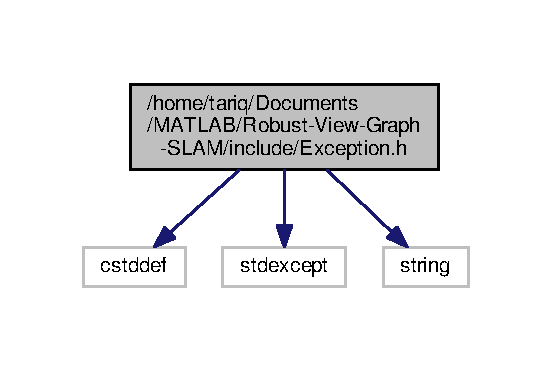
\includegraphics[width=265pt]{Exception_8h__incl}
\end{center}
\end{figure}
This graph shows which files directly or indirectly include this file\+:\nopagebreak
\begin{figure}[H]
\begin{center}
\leavevmode
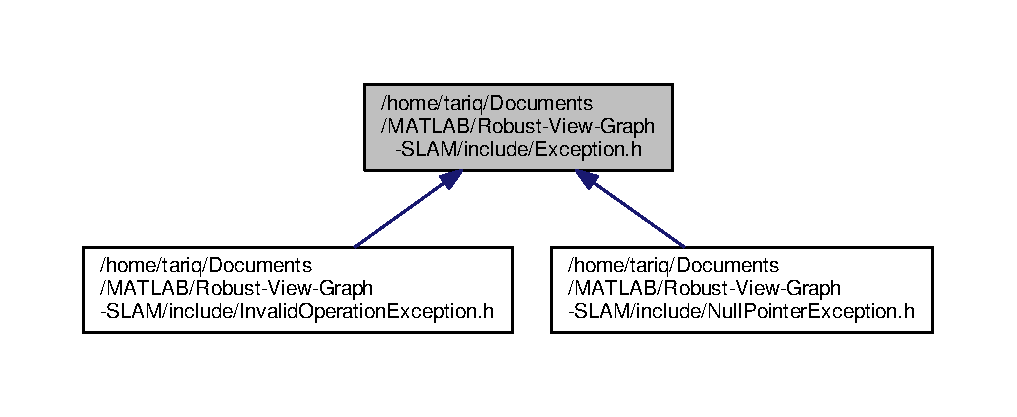
\includegraphics[width=350pt]{Exception_8h__dep__incl}
\end{center}
\end{figure}
\subsection*{Classes}
\begin{DoxyCompactItemize}
\item 
class \hyperlink{classException}{Exception}
\begin{DoxyCompactList}\small\item\em \hyperlink{classException}{Exception} base class. \end{DoxyCompactList}\end{DoxyCompactItemize}


\subsection{Detailed Description}
This file defines the \hyperlink{classException}{Exception} class, which is the base class for all exceptions. 


\hypertarget{InvalidOperationException_8h}{}\section{/home/tariq/\+Documents/\+M\+A\+T\+L\+A\+B/\+Robust-\/\+View-\/\+Graph-\/\+S\+L\+A\+M/include/\+Invalid\+Operation\+Exception.h File Reference}
\label{InvalidOperationException_8h}\index{/home/tariq/\+Documents/\+M\+A\+T\+L\+A\+B/\+Robust-\/\+View-\/\+Graph-\/\+S\+L\+A\+M/include/\+Invalid\+Operation\+Exception.\+h@{/home/tariq/\+Documents/\+M\+A\+T\+L\+A\+B/\+Robust-\/\+View-\/\+Graph-\/\+S\+L\+A\+M/include/\+Invalid\+Operation\+Exception.\+h}}


This file defines the \hyperlink{classInvalidOperationException}{Invalid\+Operation\+Exception} class, which represents invalid operations exceptions.  


{\ttfamily \#include $<$cstddef$>$}\\*
{\ttfamily \#include $<$string$>$}\\*
{\ttfamily \#include \char`\"{}Exception.\+h\char`\"{}}\\*
Include dependency graph for Invalid\+Operation\+Exception.\+h\+:\nopagebreak
\begin{figure}[H]
\begin{center}
\leavevmode
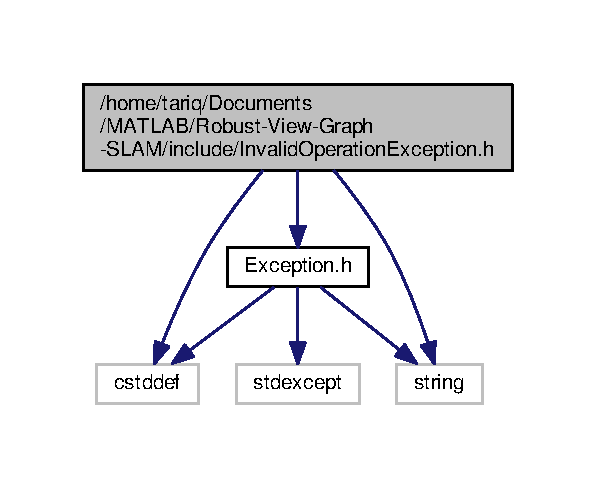
\includegraphics[width=286pt]{InvalidOperationException_8h__incl}
\end{center}
\end{figure}
\subsection*{Classes}
\begin{DoxyCompactItemize}
\item 
class \hyperlink{classInvalidOperationException}{Invalid\+Operation\+Exception}
\begin{DoxyCompactList}\small\item\em Invalid operation exception. \end{DoxyCompactList}\end{DoxyCompactItemize}


\subsection{Detailed Description}
This file defines the \hyperlink{classInvalidOperationException}{Invalid\+Operation\+Exception} class, which represents invalid operations exceptions. 


\hypertarget{NullPointerException_8h}{}\section{/home/tariq/\+Documents/\+M\+A\+T\+L\+A\+B/\+Robust-\/\+View-\/\+Graph-\/\+S\+L\+A\+M/include/\+Null\+Pointer\+Exception.h File Reference}
\label{NullPointerException_8h}\index{/home/tariq/\+Documents/\+M\+A\+T\+L\+A\+B/\+Robust-\/\+View-\/\+Graph-\/\+S\+L\+A\+M/include/\+Null\+Pointer\+Exception.\+h@{/home/tariq/\+Documents/\+M\+A\+T\+L\+A\+B/\+Robust-\/\+View-\/\+Graph-\/\+S\+L\+A\+M/include/\+Null\+Pointer\+Exception.\+h}}


This file defines the \hyperlink{classNullPointerException}{Null\+Pointer\+Exception} class, which represents null pointer exceptions.  


{\ttfamily \#include $<$cstddef$>$}\\*
{\ttfamily \#include $<$string$>$}\\*
{\ttfamily \#include \char`\"{}Exception.\+h\char`\"{}}\\*
Include dependency graph for Null\+Pointer\+Exception.\+h\+:\nopagebreak
\begin{figure}[H]
\begin{center}
\leavevmode
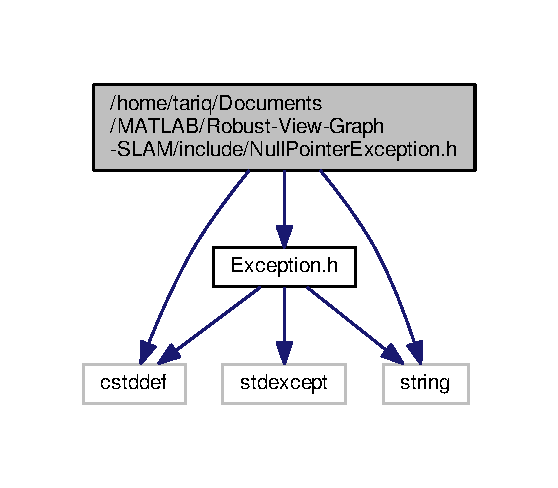
\includegraphics[width=268pt]{NullPointerException_8h__incl}
\end{center}
\end{figure}
\subsection*{Classes}
\begin{DoxyCompactItemize}
\item 
class \hyperlink{classNullPointerException}{Null\+Pointer\+Exception}
\begin{DoxyCompactList}\small\item\em Null pointer exception. \end{DoxyCompactList}\end{DoxyCompactItemize}


\subsection{Detailed Description}
This file defines the \hyperlink{classNullPointerException}{Null\+Pointer\+Exception} class, which represents null pointer exceptions. 


\hypertarget{PwgOptimiser_8h}{}\section{/home/tariq/\+Documents/\+M\+A\+T\+L\+A\+B/\+Robust-\/\+View-\/\+Graph-\/\+S\+L\+A\+M/include/\+Pwg\+Optimiser.h File Reference}
\label{PwgOptimiser_8h}\index{/home/tariq/\+Documents/\+M\+A\+T\+L\+A\+B/\+Robust-\/\+View-\/\+Graph-\/\+S\+L\+A\+M/include/\+Pwg\+Optimiser.\+h@{/home/tariq/\+Documents/\+M\+A\+T\+L\+A\+B/\+Robust-\/\+View-\/\+Graph-\/\+S\+L\+A\+M/include/\+Pwg\+Optimiser.\+h}}


Contains functions for multiple views pairwise geometry estimation.  Implements functions needed for robust nonlinear least-\/squares batch S\+L\+AM.  


{\ttfamily \#include \char`\"{}Recover\+Moments.\+h\char`\"{}}\\*
{\ttfamily \#include $<$unistd.\+h$>$}\\*
{\ttfamily \#include \char`\"{}eigen3/\+Eigen/\+Sparse\char`\"{}}\\*
{\ttfamily \#include \char`\"{}eigen3/\+Eigen/\+Dense\char`\"{}}\\*
Include dependency graph for Pwg\+Optimiser.\+h\+:\nopagebreak
\begin{figure}[H]
\begin{center}
\leavevmode
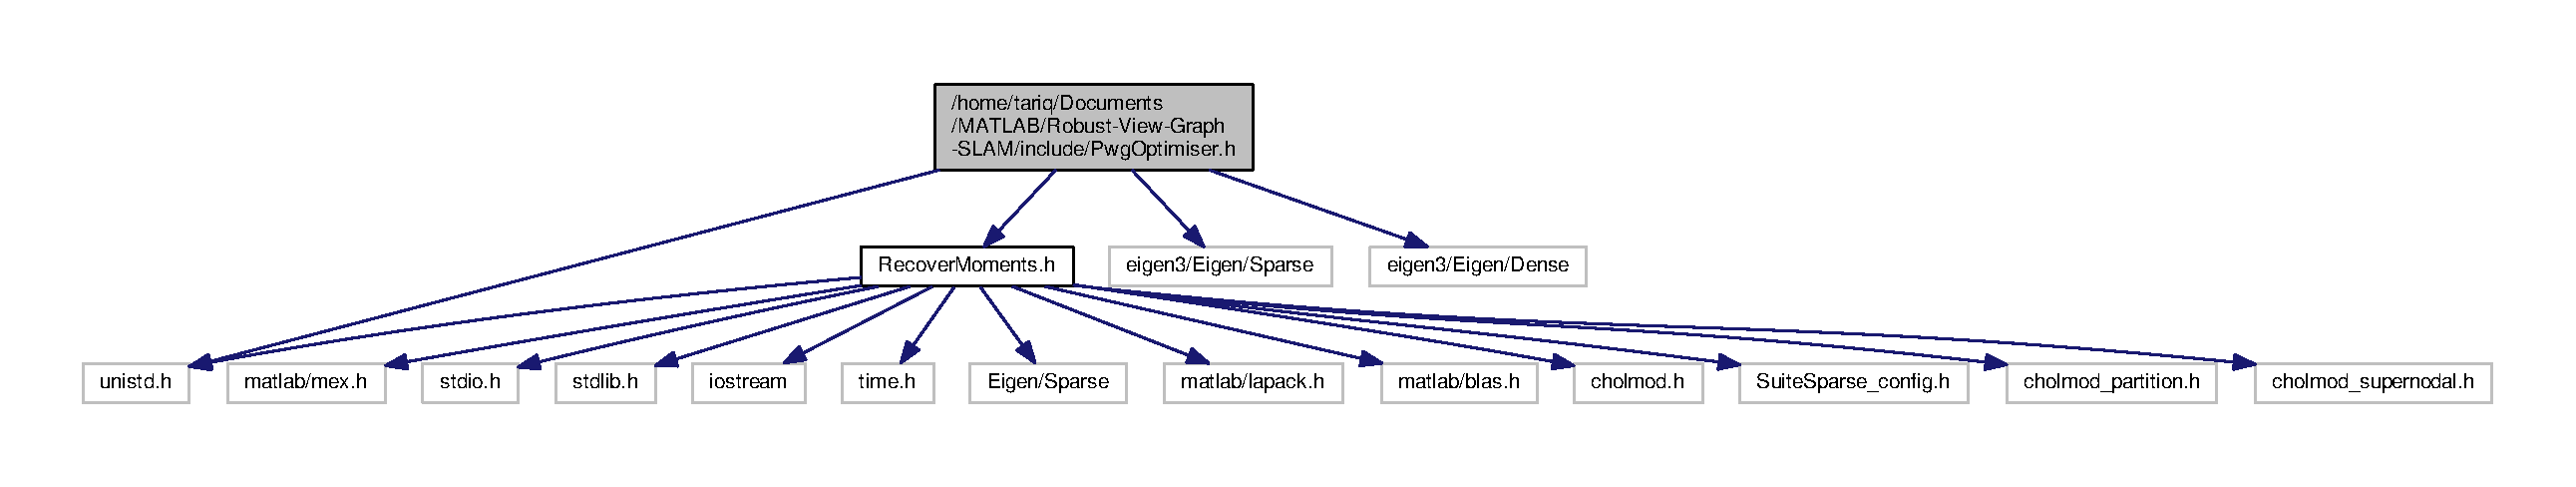
\includegraphics[width=350pt]{PwgOptimiser_8h__incl}
\end{center}
\end{figure}
\subsection*{Classes}
\begin{DoxyCompactItemize}
\item 
class \hyperlink{classPwgOptimiser}{Pwg\+Optimiser}
\item 
struct \hyperlink{structPwgOptimiser_1_1pulled__constraint}{Pwg\+Optimiser\+::pulled\+\_\+constraint}
\end{DoxyCompactItemize}
\subsection*{Typedefs}
\begin{DoxyCompactItemize}
\item 
typedef Eigen\+::\+Sparse\+Matrix$<$ double $>$ {\bfseries Sp\+Mat}\hypertarget{PwgOptimiser_8h_a04b63929a2578b5ce61f09f0b8b18122}{}\label{PwgOptimiser_8h_a04b63929a2578b5ce61f09f0b8b18122}

\item 
typedef Eigen\+::\+Triplet$<$ double $>$ {\bfseries T}\hypertarget{PwgOptimiser_8h_af639fb96631ba0018f0b2259fc95edfb}{}\label{PwgOptimiser_8h_af639fb96631ba0018f0b2259fc95edfb}

\end{DoxyCompactItemize}


\subsection{Detailed Description}
Contains functions for multiple views pairwise geometry estimation.  Implements functions needed for robust nonlinear least-\/squares batch S\+L\+AM. 

\begin{DoxyCopyright}{Copyright}
Copyright (C) 2016 i\+Cub Facility -\/ Istituto Italiano di Tecnologia 
\end{DoxyCopyright}
\begin{DoxyAuthor}{Author}
Tariq Abuhashim 
\end{DoxyAuthor}
\begin{DoxyParagraph}{email\+:}
\href{mailto:t.abuhashim@gmail.com}{\tt t.\+abuhashim@gmail.\+com} 
\end{DoxyParagraph}
\begin{DoxyDate}{Date}
Nov 2016 
\end{DoxyDate}
\begin{DoxyParagraph}{Acknowledgement\+:}
This research has received funding from the European Union’s Seventh Framework Programme for research, technological development and demonstration under grant agreement No. 611909(Koroi\+Bot). 
\end{DoxyParagraph}
\begin{DoxyParagraph}{License\+:}
Released under the terms of the L\+G\+P\+Lv2.\+1 or later, see L\+G\+P\+L.\+T\+XT 
\end{DoxyParagraph}

%--- End generated contents ---

% Index
\backmatter
\newpage
\phantomsection
\clearemptydoublepage
\addcontentsline{toc}{chapter}{Index}
\printindex

\end{document}
